\section{Related Work and Background}

\subsection{Related Work}
\begin{figure*}[!t]
\centering
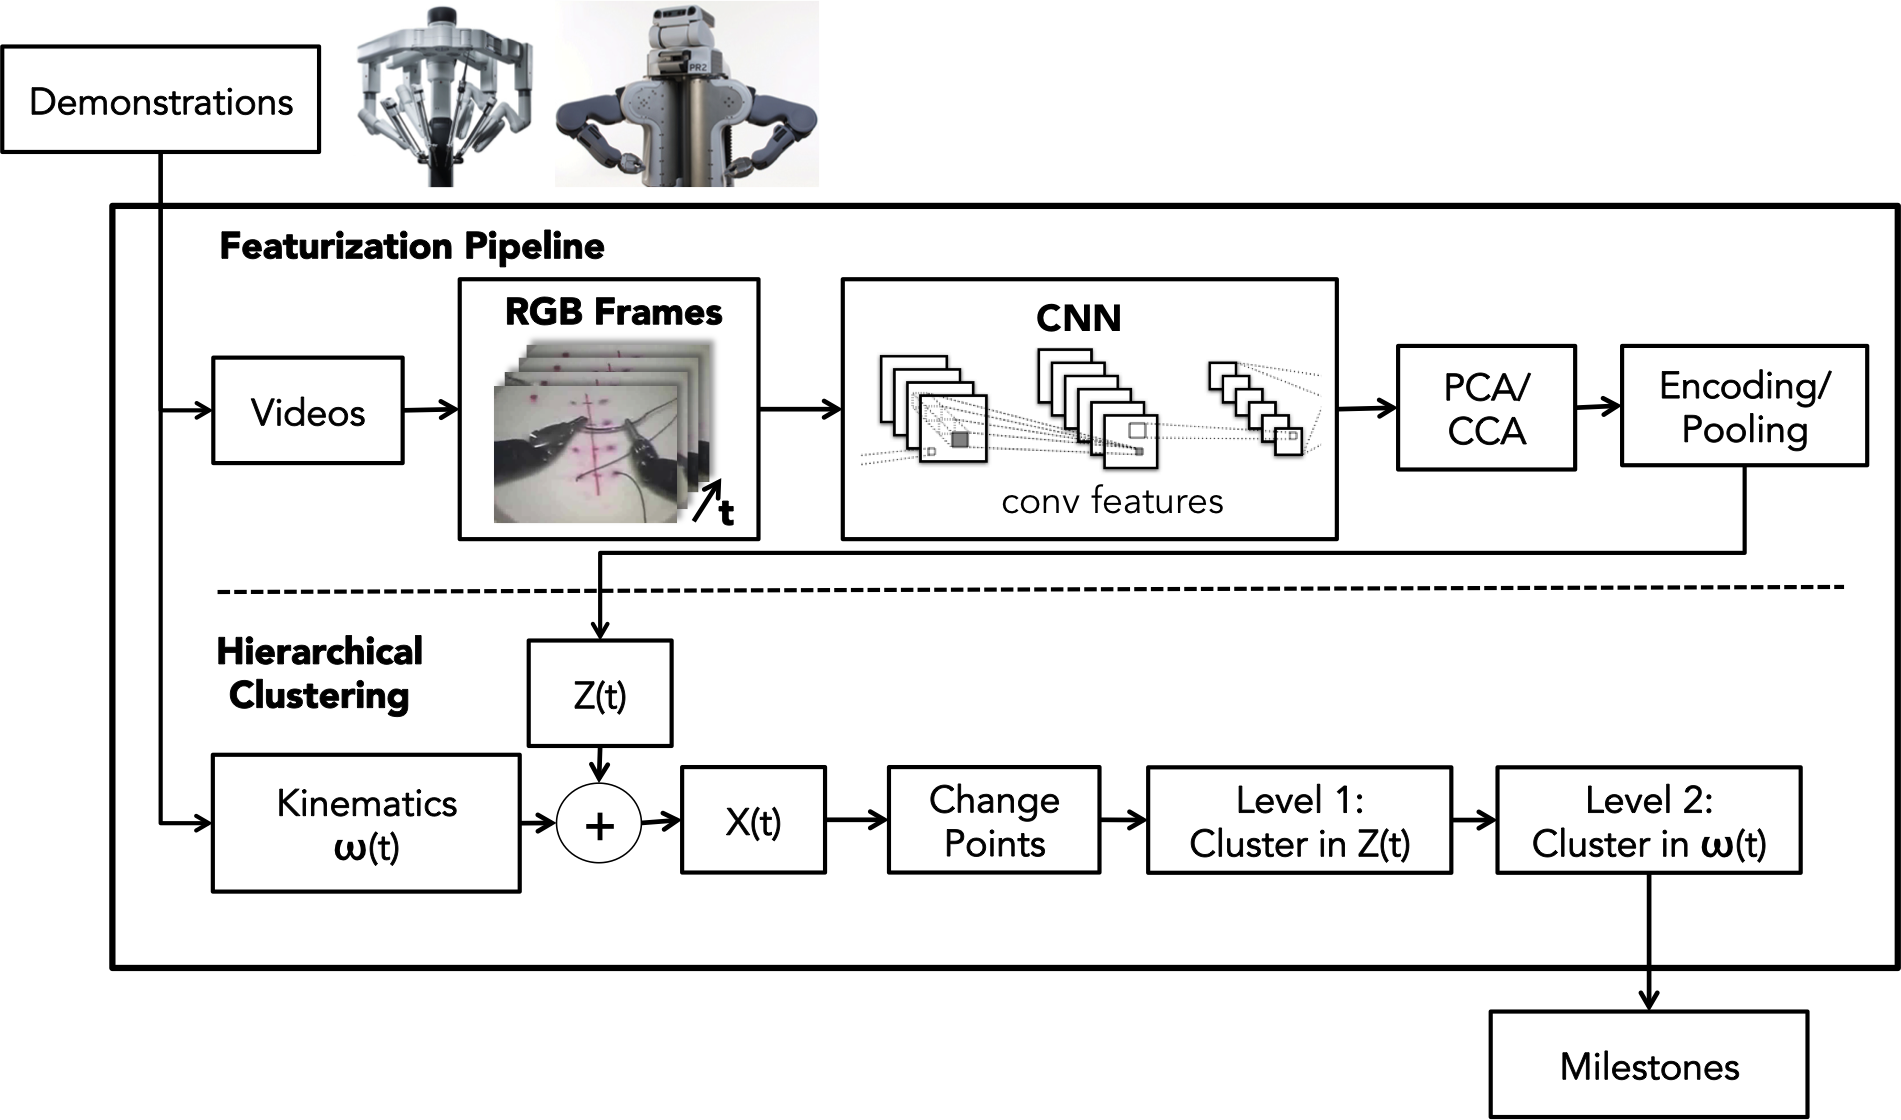
\includegraphics[width=0.7\linewidth]{figures/system_architecture_2.png}
\caption{\todo{re-draw} The figure illustrates the steps in our approach to perform seub-task level segmentation of task demonstrations without labels.}
\label{fig:pipeline}
\vspace{-10pt}
\end{figure*}

\subsubsection{Learning From Demonstrations}
Learning from demonstrations uses segmentation to discretize action spaces (skill-learning) which allows for efficient learning of complex tasks~\cite{ijspreet2002learning,pastor2009learning}.
This line of work largely focuses on pre-defined primitives.
Niekum et al. \cite{niekum2012learning} proposed an unsupervised extension to the motion primitive model by learning a set of primitives using the Beta-Process Autoregressive Hidden Markov Model (BP-AR-HMM).
The work by Niekum et al. does incorporate visual information, however, it does not use visual information to actually find segments.
Post segmentation,  Niekum et al. uses AR markers to estimate object poses of all of the objects in the workspace.
The segments, discovered with kinematics alone, are then specified in each objects reference frame.
When the objects are then moved, the trajectory can be transferred using a Dynamic Motion Primitive model.

Calinon et al.~\cite{calinon2014skills, calinon2014task, calinon2010learning} characterizes segments from demonstrations as skills that can be used to parametrize imitation learning.
In this line work, the authors apply Gaussian Mixture Models (GMMs) to cluster observations from the same mixture component.
A number of other works have leveraged this model for segmentation e.g., \cite{konidaris2009efficient, konidaris2011robot, subramanian2011learning}.
While this work does not use vision, many of the salient ideas and models are highly relevant to this paper.
As we will later describe, Gaussian Mixture Models have a duality with switched linear dynamical systems \cite{moldovan2013dirichlet}.
In this paper, we will provide experimental evidence that suggests after appropriate dimensionality reduction visual features are similar to locally linear trajectories.

\subsubsection{Surgical Robotics}
A domain of particular interest is surgical robotics which has a number of challenges that make segmentation difficult (see Krishnan et al. \cite{krishnan2015tsc}).
In our prior work, we explored automation of surgical subtasks \cite{murali2015learning} using a learning by observation framework. 
A key step in this pipeline was building a finite state machine for automation, requiring us to decompose the complex task into a small number of discrete task states.
A natural problem was to automatically segment these demonstrations algorithmically \cite{krishnan2015tsc}.
In Krishnan et al. \cite{krishnan2015tsc}, we found that hand-annotated visual features could significantly improve segmentation accuracy.

Other surgical robotics works have largely studied the problem of supervised segmentation using either segmented examples or a pre-defined dictionary of motions (similar to motion primitives).
For example, given manually segmented videos, Zappella et al. \cite{zappella2013surgical} use features from both the videos and kinematic data to classify surgical motions.
Simiarly, Quellec et al. \cite{quellec2014segmentation} use manually segmented examples as training for segmentation and recognition of surgical tasks based on archived cataract surgery videos. 
The dictionary-based approaches are done with a domain-specific set of motion primitives for surgery called ``surgemes".
A number of works (e.g., \cite{lin2005automatic, varadarajan2009data,tao2013surgical,lea15improved}), use the surgemes to bootstrap learning segmentation.

\subsubsection{Visual Gesture Recognition}
Another relevant line of work is human motion analysis and gesture recognition.
A number of recent works, attempt to segment human motions from videos \cite{hoai2011joint, tang2012learning, yang2013discovering, jones2014unsupervised, wu2014leveraging, wu2015watch}.
Tang et al. and Hoai et al. proposed supervised models for human action segmentation from video.
Building on the supervised models, there are a few unsuperivsed models for segmentation of human actions: Jones et al.\cite{jones2014unsupervised}, Yang et al. \cite{yang2013discovering}, Di Wu et al. \cite{wu2014leveraging} , and Chenxia Wu et al. \cite{wu2015watch}.
Jones et al. \cite{jones2014unsupervised} restricts their segmentation to learning from two views of the dataset (i.e., two demonstrations).
Yang et al. \cite{yang2013discovering} and Wu et al.  \cite{wu2015watch} use k-means to learn a dictionary of primitive motions, however, in prior work, we found that \sys outperforms a standard k-means segmentation approach.
In fact, the model that we propose is complementary to these works and \sys would be a robust drop-in-replacement for the k-means dictionary learning step.
The approach taken by Di Wu et al. is to parametrize human actions using a skeleton model, and they learn the parameters to this skeleton model using a deep neural network.
In this work, we explore using generic deep visual features for robotic segmentation without requiring task-specific optimization such as skeleton or action models using in human action recognition.

\subsubsection{Deep Features Robotics}
Robotics is increasingly using deep features for visual sensing. For example, Lenz et al. uses pre-trained neural networks for object detection for grasping \cite{lenz2015deep}.
Levine et al. \cite{levine2015end} fine-tune pre-trained CNNs for policy learning.
For this reason, we decide to explore the architectural design space of using deep features for trajectory modeling.
We believe that segmentation is an important first step in a number of robot learning applications, and the appropriate choice of visual features is key to accurate segmentation.
In our experiments, we numerate a number of different design choices and show how that a suboptimal (but ostensibly sensible) choice of features results in a factor of 3x less accuracy.

\subsection{Trajectory Segmentation Models}
There are a number of different ways to formalize segmentation, and we overview some of the prior work (including ours) to contextualize the results in the rest of the paper.
Many unsupervised segmentation models either implicitly or explicitly model the dynamics as locally linear.
It is important to note that locally linear dynamics does not imply linear motions, as spiraling motions can be represented as linear systems. 
In \cite{elhamifar2009sparse}, videos are modeled as transitions on a lower-dimensional linear subspace and segments are defined as changes in these subspaces.
Willsky et al~\cite{willsky2009sharing} proposed BP-AR-HMM, which was applied by Niekum et al. in robotics \cite{niekum2012learning}.
This model is explicitly linear by fitting a autoregressive model to time-series, where time $t+1$ is a linear function of times $t-k,\ldots, t$, to windows of data. 
The linear function switches according to an HMM with states parametrized by a Beta-Bernoulli model (i.e., Beta Process). 
In fact, even the works that apply Gaussian Mixture Models for segmentation \cite{calinon2010learning, lee2015autonomous, kruger2012imitation}, implicitly fit a locally linear dynamical model.
Moldovan et al. \cite{moldovan2013dirichlet} proves that a Mixture of Gaussians model is equivalent to Bayesian Linear Regression; i.e., when applied to a time window it fits a linear transition between the states.

An important challenge in this field is coping with temporal inconsistencies.
One approach is to simultaneously learn a probabilistic transition grammar with Finite State Markov Chain model with Gaussian Mixture Emissions (GMM+HMM) \cite{asfour2006imitation,calinon2004stochastic,kruger2010learning, vakanski2012trajectory}.
These models, also called Baum-Welch models, impose a probabilistic grammar on the segment transitions and can be learned with an EM algorithm.
However, they can be sensitive to hyper-parameters such as the number of segments and the amount of data \cite{tang2010toward}.
The problem of robustness in GMM+HMM (or closely related variants) has been addressed using down-weighting transient states \cite{kulic2008scaffolding} and sparsification \cite{grollman2010incremental}.

In prior work, we propose \sys to address the challenge of robust unsupervised segmentation.
Ultimately, the model was a hierarchical application of a Dirichlet Process-Gaussian Mixture model.
After a series of merging and pruning steps, the resulting segments showed increased robustness to temporal variation and outliers.
In this work, we extend this model to account for visual features in the robot state.

